\chapter{Changes of Cloud Radiative Effect to Global Warming}
\label{ch:cld_fbk}

In \chapref{ch:simple_cld_scheme}, we have introduced how the simple cloud scheme is constructed, and have evaluated the simulated climatology when it is implemented in Isca. The simulations have shown that it can grasp the basic features of cloud climatology. In this chapter, the simulated cloud feedbacks under global warming are to be examined. Also, based on this simple cloud scheme, a series of perturbed parameter ensemble (PPE) experiments are carried out to investigate whether they can `reproduce' the inter-model spread of cloud feedbacks among CMIP models. Based on the results, the sensitivities of the corresponding parameters, components and processes are analyzed. The cloud controlling factor analysis are employed to identify the possible causes for the cloud responses.

The major findings of this chapter are

\begin{enumerate}
    \item The simulated cloud feedback from the simple cloud scheme is generally reasonable, but failed to grasp the strong negative optical depth feedback in Southern Ocean regions, as the ice condensate is not explicitly represented in the simple cloud scheme.
    \item The low cloud amount feedback is the single largest contributor to the net cloud feedback spread of the PPE, which is consistent with the inter-model spread of CMIP models.
    % consistent with previous studies such as \cite{Bony2005, Zelinka2016insights}.
    \item The regions abundant of stratocumulus clouds show negative feedback in the simulations, as the low cloud component of the simple cloud scheme depends too strongly on the inversion strength.
    \item For ECS, ...
\end{enumerate}

\section{Introduction}

% What is cloud feedback and why it is important
As introduced in \chapref{ch:introduction} and \chapref{ch:simple_cld_scheme}, clouds heat the Earth by absorbing and re-emitting the longwave radiation, and cool the Earth by reflecting the incoming solar radiation, the so called cloud radiative effect. In total, the net radiative effect of clouds is to cool the Earth at the magnitude about 20 Wm$^2$ (\figref{fig:CRE_from_IPCC}). But the problem about how the cloud radiative effect would change under global warming (i.e., cloud feedback) has haunted climate community for decades. For example, in early 1990s, \cite{Cess1990intercomparison} evaluated the climate feedback processes in 19 Atmospheric General Circulation Models (AGCMs), and found that the broad spectrum of cloud feedbacks (from modest negative to strong positive) is the consequence of the models' different responses to sea surface temperature warming. Also, models may have similar responses if their net cloud feedbacks are similar, despite of large difference in their compensating solar or infrared components. Later, an updated analysis in AGCMs suggest that the models have moderate net cloud feedbacks compared to their predecessors, but these changes can be traced to different treatments of clouds in the respective models, and the spread of shortwave and longwave cloud feedback components is still substantial, indicating that the models still have physical disagreements \citep{Cess1996cloud}. Other studies such as \cite{Colman2003comparison}, \cite{Webb2006contribution} and \cite{Vial2013} also concluded that differences in cloud feedback make a large contribution to differences in climate sensitivity in GCMs. In recent CMIP6 models, the mutli-model mean net cloud feedback is positive \citep[see \figref{fig:zelinka_global_mean_fbks};][]{Zelinka2020causes}, meaning that the cloud would cool the planet less than before as the planet warms. Nevertheless, the cloud feedback still has the largest uncertainty among all the climate feedback parameters,  remaining the leading cause for the inter-model spread of equilibrium climate sensitivity (ECS) in climate models \citep{Zelinka2020causes,Sherwood2020}. %Cess1990intercomparison,Cess1996cloud,Webb2006contribution,Vial2013,

% Why the spread is so large?

Over the years, the climate community has been focusing on understand the underlying causes of the spread in cloud feedbacks among the models, and trying to reduce such spread so as to minimize the potential range of ECS. Both in observation and models, the frequencies of occurrence of different cloud types are unequal  \citep[e.g.,][]{Zhang2005comparing}, and so the behaviors of certain clouds may matter than that of others in explaining the range of cloud feedbacks among models \citep{Bony2006}. For example, \cite{Wyant2006comparison} show that the responses of deep convective clouds and of low-level clouds differ among climate models. 
Previous studies suggested that among all the cloud feedbacks, the tropical low cloud feedback is regarded as the major contributor for the inter-model spread 
\citep[e.g.,][]{Bony2005,Webb2006contribution,Webb2013coupling,Vial2013,Zelinka2016insights}. For example, \cite{Bony2005} decomposed the tropical ocean region into different dynamical regimes by vertical velocity with the method proposed by \cite{Bony2004}, showing that the cloud radiative effects differ most in subsidence regimes among CMIP3 models, suggesting a dominant role of low clouds in driving the spread of tropical cloud feedbacks. \cite{Webb2006contribution} also confirmed the role of low clouds by analyzing the cloud feedbacks in the doubling-CO$_2$ slab-ocean experiments from nine CFMIP models, and found that differences in cloud feedbacks in low cloud areas make the largest contribution to the spread in the global feedback. The findings are also confirmed in CMIP5 models. For instance, \cite{Vial2013} quantified the inter-model spread of climate sensitivity and decomposed it into contributions from individual adjustments and feedbacks, and into regional contributions (i.e., tropical, mid-latitude and polar regions). They estimated that about 70 \% of the inter-model spread in climate sensitivity stems from cloud feedbacks, among which tropical region plays the largest role. After breaking down the tropical changes into dynamical and thermodynamical components \citep[method from][]{Bony2004}, they found the  thermodynamic component is in fact the major source of the spread in tropical cloud feedbacks. In recent years, \cite{Zelinka2012computing1,Zelinka2012computing2} proposed a refined decomposition of cloud feedbacks, the so called `cloud radiative kernel method' (to be described in detail later; also in \secref{sec:method_cloud_fbk}), in which the cloud feedback can be decomposed into cloud amount, altitude and optical depth feedbacks. Through this method, \cite{Zelinka2016insights} identified the low cloud amount feedback is the single largest contributor to the spread in net cloud feedback, although the non-low clouds also play certain roles in driving the spread of cloud feedbacks. 
%treated the tropospheric adjustments to CO$_2$ and land surface warming as part of forcings rather than feedbacks, and used the radiative kernel method to decompose the total climate feedback into different components. 

%The amplitude and inter-model spread of climate sensitivity is quantified, and decomposed into different contributions related to individual adjustments and feedbacks, and into regional contributions.\citep[e.g.,][]{Vial2013,Zelinka2016insights}.

%\cite{Zelinka2016insights} also suggest the high-clouds also play certain role in the spread of cloud feedbacks among CMIP models.

% How to quantify the cloud feedbacks
To understand the underlying causes for the spread of cloud feedbacks, we need to quantify the cloud feedbacks first, which is the necessary basis for the future analysis. As introduced in \secref{sec:method_cloud_fbk}, several approaches have been used previously to calculate the cloud feedbacks in GCMs. The idea of these methods is to quantify the change of cloud radiative effect in response to unit change of global mean surface temperature. The intuitive way is to calculate the change of cloud radiative effect under control and perturbed experiments, and normalized the changes by the global mean surface air temperature \citep[e.g.,][]{Cess1990intercomparison,Cess1996cloud}. However, this may be not an accurate estimate of the change of cloud radiative effect, as  the non-cloud induced changes are also included \cite[e.g.,][]{Soden2004}. Of course, the so called cloud-masking effect can be removed using the all-sky and clear-sky radiative kernels \citep[Details in \secref{sec:method_cloud_fbk}][]{Shell2008}. In addition, as pointed by \cite{Soden2008} and \cite{Vial2013}, this method in fact can reflect the spread of cloud feedbacks although the magnitude or sign may not be reasonable, and that is why it is still widely used in recent studies \citep[e.g.,][]{Webb2015}. Another possible problem of this approach is that it can obtain the total changes of cloud radiative fluxes at TOA, but could not identify from which type of clouds that these radiative fluxes changes arise. As the cloud location and optical properties (e.g., thin or thick) are essential to understand the possible changes in cloud longwave and shortwave radiative effects. Another type of approaches employed in previous studies are the partial radiative perturbation (PRP) method \citep{Wetherald1988cloud} and its variations such as two-way PRP \citep[e.g.,][]{Colman1997} and radiative kernel method \citep[e.g.,][]{Soden2008,Shell2008,Huang2017,Pendergrass2018,Smith2020}. This kind of method quantifies the partial derivation of TOA radiation flux with respect model parameters such as temperature, water vapor and clouds. The traditional PRP method is quite computing expensive, while the radiative kernel method can calculate the kernels in advance and be applied to many different GCM situations. The method is useful to explicitly decompose the climate feedbacks into various components, and can help us evaluate the cloud feedback alone \citep[e.g.,][]{Soden2004,Soden2006,Soden2008}. Taking the masking effect into consideration, one can get the longwave and shortwave parts of cloud feedback from this method \citep[e.g.,][]{Soden2008,Caldwell2016quantifying}, but it is hard to decompose the cloud feedback in further into refined constituents, as the radiative kernels provided by some GCMs such as CAM5 \citep{Pendergrass2018} and HadGEM \citep{Smith2020} are limited to all-sky and clear-sky temperature and water vapor, and surface albedo kernels. Of course, one can generate such kernels for cloud water and other components, but it is not easy to implement, which is a limitation of this approach. In recent years, a new technique called cloud radiative kernel method is proposed by \cite{Zelinka2012computing1,Zelinka2012computing2}, which can be regarded as a variation of PRP method applied to the joint histogram of cloud top pressure and optical depth from ISCCP simulator \citep{Klein1999validation,Webb2001combining}. With this approach, the TOA radiative flux changes can be attributed to specific cloud types, and can be partitioned into specific changes in amount, altitude and optical depth. Moreover, as the kernel is derived from the cloud related fields only, the calculation is not impacted by clear-sky changes that are irrelevant to cloud feedback, so the derived TOA flux changes are due to the change of clouds only. It has shown that this refined decomposition can provide some insights for understanding the spread of cloud feedbacks in GCMs \citep[e.g.,][]{Zelinka2016insights,Zelinka2020causes,Zelinka2021evaluating}.

The cloud feedback calculation and decomposition methods mentioned above are used to answer the first question that we are going to explore in this chapter, that is whether the simple cloud scheme described in \chapref{ch:simple_cld_scheme} could grasp the key mechanisms of cloud feedbacks. The results in \chapref{ch:simple_cld_scheme} show that this simple cloud scheme could grasp a relatively reasonable cloud climatology, but as pointed by \cite{Zelinka2021evaluating} that better simulation of mean-state cloud properties does not necessarily guarantee the better simulation of cloud feedbacks. To do so, the performance of the simple cloud scheme in simulating the cloud feedbacks are to be evaluated in this chapter and compared to CMIP5/6 GCMs and the expert assessments from \cite{Sherwood2020}. 

Another followed question is whether we could reproduce a certain level of spread in cloud feedback by perturbing a series of physical parameters in the simple cloud scheme. As the perturbed physics ensemble (PPE) is a widely used method to understand the uncertainty of GCMs. For example, \cite{Murphy2004quantification} performed a systematic attempt to determine the range of climate sensitivity based on a 53-member ensemble of model versions constructed by varying the subset of all the model physical parameters. \cite{Webb2013origins} investigated the origins of differences in climate sensitivity, forcing and climate feedbacks with the multi-model ensemble of CMIP3 models and 15 perturbed parameter ensemble members of HadGEM3 slab model, and they found that the cloud feedback uncertainty is about twice of the role of cloud forcing in determining the spread of climate sensitivity, and the low latitude ocean region contributes more than other areas. Inspired by these results, here we also seek to examine the uncertainty of cloud feedbacks by varying the physical parameters in Isca model, and the only difference is that our perturbation is only limited to cloud scheme, while the parameters from other physical processes such as convection are kept unchanged. In doing so, we expect the spread of cloud feedback would be smaller compared to the inter-model range of CMIP models, and also likely smaller than the PPEs in which parameters from all the physical schemes are perturbed, but it could be easier for us to identify which parameter or process in cloud scheme is most sensitive. Morover, if the PPE of Isca simulations can produce certain spread of cloud feedbacks, what are the underlying causes for this uncertainty? Are they similar to those of CMIP models? These are the problems we need to answer through the PPE results in this chapter.

%which parameter or process is most sensitive?
%In this chapter, the following questions are going to be answered. First, could the simple scheme grasp the key mechanisms for cloud feedback? The results in \chapref{ch:simple_cld_scheme} have shown that the simple cloud scheme could grasp a relatively reasonable cloud, but as pointed by \cite{Zelinka2021evaluating} that better simulation of mean-state cloud properties does not necessarily guarantee better cloud feedbacks.

%Could we ‘reproduce’ the spread of cloud feedback by perturbing a series of physical parameters? And which parameter or process is most sensitive?

%What are the implications for equilibrium climate sensitivity?

The outline of this chapter is as follows. \secref{sec:simulation_setup_cld_fbk} describes the basic simulation setups in this chapter, including the implementation of observation satellite simulator package, the perturbed physics ensemble in Isca, and how the Q-flux is prescribed in the simulations. In \secref{sec:eval_cosp}, the behaviors of satellite simulator is examined to make sure it is correctly implemented. Then based on the satellite simulator outputs and the cloud radiative kernel method, we compared the several different methods to compute the cloud feedbacks in \secref{sec:cmp_cld_fbk_method_result}, which is the basis for our future analysis. In \secref{sec:simu_cld_fbk}, we present the simulated spatial pattern and zonal mean structures of cloud feedbacks from the PPEs, and explain the possible mechanisms for the feedbacks. The spread of cloud feedbacks from PPE of Isca simulations and the underlying causes for the spread are investigated in \secref{sec:spread_of_cld_fbk_in_PPE}. In this section, at first the global mean longwave, shortwave and net cloud feedbacks and their components decomposed by altitude and types are examined in \secref{sec:spread_of_gm_cld_fbks_PPE}, and the relative contributions of these components to spread of net cloud feedbacks are quantified. Also, these feedbacks are also evaluated against the expert assessment based on multi-line evidence from \cite{Sherwood2020}, and the reasons for the agreement and disagreement with these expert assessment are analyzed (\secref{sec:cmp_with_Sherwood_assessment}). The contributions to the spread of cloud feedback from tropical and extra-tropical regions are quantified in \secref{sec:reg_contri_to_spread_of_cldfbk}, and the possible reasons are explored by the cloud controlling factor analysis in \secref{sec:cld_control_factor}. Finally, the relationship between cloud feedback and the equilibrium climate sensitivity is investigated briefly in \secref{sec:implification_for_ECS}.


\section{Simulation setup}
\label{sec:simulation_setup_cld_fbk}
%Similar to the setups in \secref{sec:eval_cld_exp_setup}, here the SST has a uniform 4K warming.

\subsection{Implementation of the COSP}

As introduced in \secref{sec:Zelinka_method}, one possible way to calculate the cloud feedback is to use the cloud radiative kernel \citep{Zelinka2012computing1,Zelinka2012computing2}, in which the joint-histogram between cloud top pressure and optical depth from ISCCP cloud simulator \citep{Klein1999validation,Webb2001combining} is needed. One can simply estimate the cloud feedback by the change of cloud radiative effect between control and perturbed experiments, but it also includes the masking effect of climatological cloudiness on non-cloud feedbacks \citep{Soden2004}. In addition, combining the histogram outputs from ISCCP cloud simulator with cloud radiative kernel, one can decompose the cloud feedback into  different altitude and different components \citep{Zelinka2012computing2,Zelinka2016insights}, which is a helpful tool for us to understand the causes of spread in multi-model spread of cloud feedback. As mentioned in \secref{ch:simple_cld_scheme}, the cloud simulator has not been implemented in Isca, and we could not employ the cloud radiative kernel method to calculate and decompose cloud feedback without it. Thus in this section, we try to implement the cloud simulator in Isca first in order for a refined look into cloud feedback.

As introduced in \chapref{ch:methods}, the Cloud Feedback Model Intercomparison Project (CFMIP) Observational Simulator Package (COSP) version 2 \citep{Swales2018} is implemented in Isca. The satellite simulator is a kind of diagnostic code applied to model variables, aiming to reduce the inconsistencies between the ways clouds are observed by satellites and the ways they are simulated in models \citep{BodasSalcedo2011}. From the satellite simulator, one can obtain what a satellite would retrieve if the atmosphere had the clouds of the model in the real world. In addition, it also facilitates intercomparison among GCMs by minimizing the impacts of how clouds are parameterized in models \citep[e.g.][]{Klein2013climate}. The extremely thin clouds (i.e., $\tau<$0.3) are excluded in the COSP analysis, as the models usually disagree largely with ISCCP observation in this category. One possible reason for this is the impact of the thin clouds on TOA radiation budget is usually difficult to detect by the passive sensors from the ISCCP satellites \citep{Klein2013climate}.

One key diagnostic output to be acquired from the COSP is the joint histogram of cloud-top pressure (CTP) and optical depth ($clisccp$ in CFMIP variables). In current setup, the histogram segments are first obtained separately for each CTP category (7 in total), and then the whole histogram is derived directly by concatenating these segments, as they are independent to each other. In the AMIP-type simulations or the ones performed with Q-flux (to be introduced in \secref{sec:PPE_setup}), the COSP is only run for the last five years, and the ISCCP simulator is enabled alone as its outputs are what we need here to calculate the cloud feedbacks. Note that the COSP is always active only in one simulation to get the kernel-derived cloud-induced radiation anomalies, so as to calculate cloud feedback through the \cite{Gregory2004} method  (see bottom right category of \tabref{tab:four_methods_cldfbk_results}). The performance of the COSP is examined in \secref{sec:eval_cosp}.

% , boundaries are 1000, 800, 680, 560, 440, 310, 180 hPa

% Possible reason of too much thick  clouds is the treatment of cloud water is not reasonable: e.g., no partition between snow and liquid water?
% vertical resolution too coarse to simulate the thin clouds?

%In this study, the Cloud Feedback Model Intercomparison Project (CFMIP) Observational Simulator Package (COSP) version 2 \citep{Swales2018}, which can be accessed at \url{https://github.com/CFMIP/COSPv2.0}, is implemented in Isca. COSP was originally developed as a satellite simulator package whose aim is to produce virtual satellite observations from atmospheric model fields for a better comparison of model output with observations \citep{Bodas2011}. This approach is needed because the satellite retrievals generally do not directly correspond to the numerical model fields due to the mismatch between their definitions of certain fields. COSP accounts for the limited view of the satellite instrument by calculating radiative transfer through the atmosphere, i.e. attenuation by hydrometeors and air molecules and backscattering \citep{Kuma2020}. Note that multiple instrument simulators, such as MODIS, CALIPSO, CloudSat and ISCCP, have been incorporated in COSP, and it is flexible for users to decide which one to use based on their research purposes. 

% Specifically, several modules have been written in Isca to call COSP, in which the outputs from simple cloud scheme and SOCRATES radiation schemes, such as cloud fraction, effective radius, cloud water content and cloud optical depth, are provided through the interfaces. However, as the cloud scheme is simple and there is not microphysics scheme in Isca, we could not provide some properties about convective clouds and cloud condensate such as ice and graupel. Although this may bring some problems, the outputs from ISCCP simulator are relatively reasonable.

% \subsection{Q-flux}
% \label{sec:Q_flux_intro}

 %As in \chapref{ch:simple_cld_scheme}, the observed SST is from the input4MIPs data set \citep{Durack2018} over the period from 1979 to 2008. To derive the Q-flux, the aforementioned SST climatology is prescribed in a simulation with the realistic continents and a slab ocean of 20m depth. The energy balance model is applied as follows:
% \begin{equation}
%     F_Q = C_w\rho_w D \frac{\partial T}{\partial t} - F_s,
%     \label{eq:Q_flux}
% \end{equation}

% \begin{equation}
%     F_s = SW-LH-SH-LW,
%     \label{eq:surface_flux}
% \end{equation}
% where $F_Q$ is the Q-flux to be derived, which distributes energy globally to match the prescribed SST distribution. The $C_w$ (3989.24 J kg$^{-1}$ K$^{-1}$) and $\rho_w$ (1035 kg m$^{-3}$) are the specific heat capacity and density of ocean water, respectively. $D$ is the depth of mixed layer. The rate of change in mixed layer temperature ($\frac{\partial T}{\partial t}$, in units of K s$^{-1}$) is calculated by the prescribed SST. The surface flux ($F_s$, positive downward, units Wm$^{-2}$) in \Eqref{eq:Q_flux} is calculated from the upward latent and sensible heat fluxes ($LH$ and $SH$, respectively), the net longwave radiation ($LW$, positive upward) and net shortwave radiation ($SW$, positive downward), as indicated by \Eqref{eq:surface_flux}.

% \begin{figure}[ht]
% 	\centering
% 	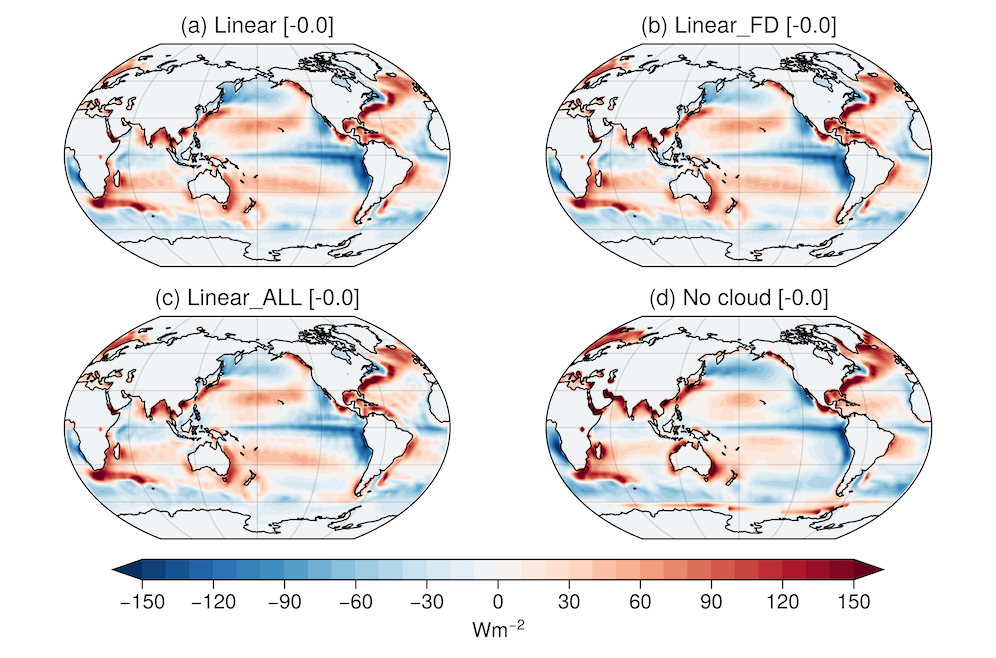
\includegraphics[width=1\linewidth]{{figs/change_of_CRE/Q-flux_cmp}.png}
% 	\caption[Comparison of spatial pattern of ocean heat transport (Q-flux).]{Annual mean Q-flux pattern (in W m$^{-2}$) derived from AMIP fixed-SST experiments with realistic continents and topography. The cloud schemes used are (a) linear, (b) linear\_FD and (c) linear\_ALL as in \tabref{tab:exps} and (d) no cloud scheme.}
% 	\label{fig:Q_flux_cmp}
% \end{figure}

% The AMIP fixed-SST experiments with linear cloud scheme described in \tabref{tab:exps} and a new fixed-SST simulation without clouds are used to derived the Q-flux, and the results are shown in \figref{fig:Q_flux_cmp}. The spatial patterns of Q-flux from different cloud schemes are similar, and have some differences from the simulation without cloud in subtropical and Southern Ocean regions. Q-flux can capture the ocean currents such as the Gulf Stream and cold tongue in the eastern tropical Pacific (\figref{fig:Q_flux_cmp}), and the positive value compensates for too little heating to the slab ocean by the surface flux from the `prescribed-SST’ run compared to the SST climatology. In this case, the Q-flux obtained from the run with the linear cloud scheme only is used in the following simulations. Also, the Q-flux remains the same in the control and perturbed experiments, but it is noted that the SST can change freely in response to different CO$_2$ forcing. 

\subsection{Perturbed parameter ensemble}
\label{sec:PPE_setup}
 
 In this chapter, the parameters of the simple cloud scheme are perturbed to
 

 \begin{table}
%\begin{sidewaystable}
	\caption{Design of the perturbed parameter experiments (PPEs). All simulations are run in T42 horizontal resolution.}
	\centering
	\renewcommand{\arraystretch}{1.5}
	\resizebox{\textwidth}{!}{
	\begin{tabular}{cc >{\raggedright}m{0.26\linewidth} m{0.6\linewidth}} 
	% control width, alignment for cells
	% https://texblog.org/2017/02/06/proper-tables-with-latex/
		\toprule
	    Index & Experiment & Parameter change & Description \\
		\midrule
		1 & Linear & Default values in \tabref{tab:cld_scheme_summary} & Simulations with Q-flux; Control (1$\times$CO$_2$) and perturbed (4$\times$CO$_2$) experiments \\
		2 & a\_surf & $a_{s}: 42 \rightarrow 20$ & Equivalent to decrease the critical relative humidity at the surface \\
		3 & a\_top & $a_{t}: 13 \rightarrow 10$ & Equivalent to decrease the critical relative humidity at the upper troposphere \\
		4 & Sc\_coeff\_c & $c: -0.1 \rightarrow -0.3$ & The added stratocumulus clouds should decrease \\
		5 & Sc\_coeff\_b & $b: 1.3 \rightarrow 1$ & The added stratocumulus clouds should decrease \\
		6 & Tmax &  $T_{max}:-5\rightarrow 0~^\circ$C & Increase the temperature threshold of the fraction of liquid cloud (Reff would increase) \\
		7 & Tmin & $T_{min}: -40\rightarrow -35~^\circ$C & Increase the temperature threshold of the fraction of ice cloud \\
		8 & Reff\_ice & $r_{e_ice}:25\rightarrow 50~\mu$m & Increase the default effective radius for ice cloud \\
		9 & Reff\_liq & $r_{e_ice}:14\rightarrow 12~\mu$m & Decrease the default effective radius for liquid cloud \\
		%rcl\_height &  & In-cloud liquid water mixing ratio is specified as a function of height, rather than as temperature \\
		10 & freezedry & On & Use the freezedry method \\
		11 & Sundqvist & On & Change the default cloud fraction scheme from linear to Sundqvist \\
		12 & cld\_water & $m_{l}=0.2$ & Increase the maximum of in-cloud water mixing ratio a box can reach \\
		%12 & qcl\_T & $q_{l}=0.2$ & In-cloud water mixing ratio as a function of height \\
		\bottomrule
	\end{tabular}
	}
	\label{tab:qflux_ppe_exps_summary}
%\end{sidewaystable}
\end{table}

 The simulations in \chapref{ch:simple_cld_scheme} are the AMIP-type fixed-SST experiments, and the changes in atmosphere could not feedback into the SST changes. To make it more realistic, here we prescribe the derived ocean heat transport flux (the `Q-flux') from a given distribution of SSTs following the method from \cite{Russell1985}, so that the SST can respond freely to the CO$_2$ forcing. The detailed description of how Q-flux is calculated can be found in \secref{sec:Q_flux_method}. 

%\section{Results}
%\label{sec:results_cld_fbk}

%In this section, the simulated cloud feedbacks from Isca are to be introduced.

%\subsection{}

\section{COSP evaluation}
\label{sec:eval_cosp}

\begin{figure}[ht]
    \centering
    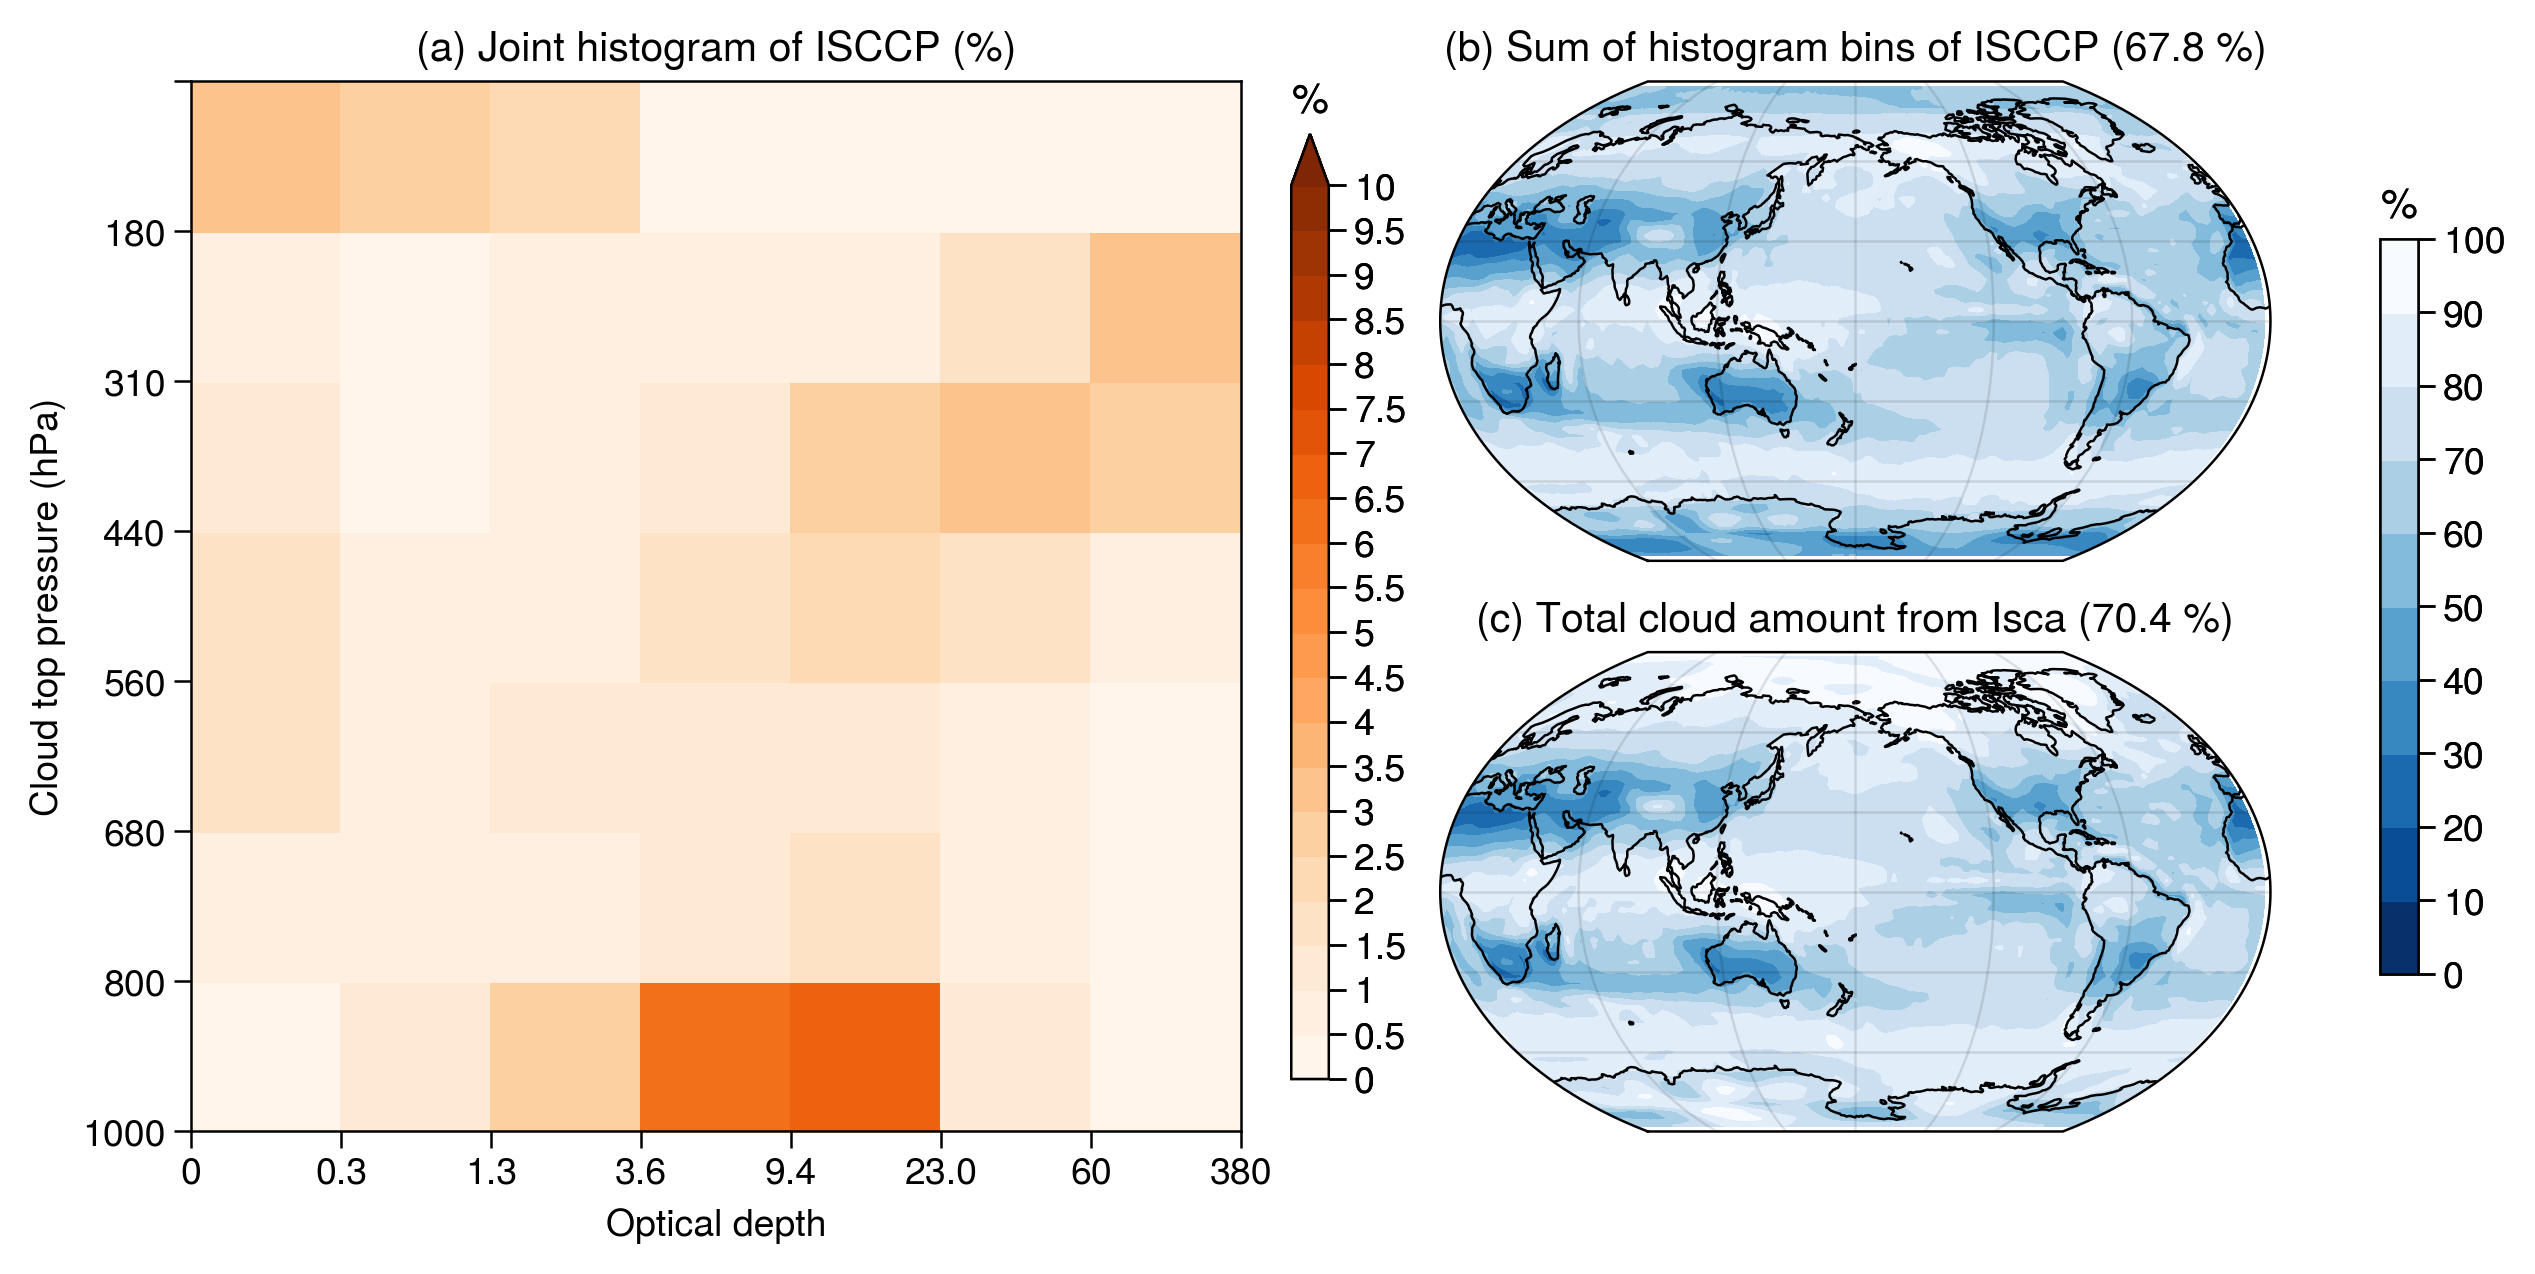
\includegraphics[width=1\linewidth]{{figs/change_of_CRE/cmp_isca_cosp_tot_cld_amt}.png}
    \caption{(a) The annual mean cloud fraction (\%) binned by the joint histogram of cloud top pressure and optical depth from ISCCP simulator implemented in Isca. (b) The sum of the histogram bins for each location from the ISCCP simulator of Isca. (c) The annual mean native total cloud amount from Isca simualtions based on max-random overlap assumption.}
    \label{fig:cmp_isca_and_sum_of_COSP}
\end{figure}

The implementation of COSP provides a new tool to compare Isca simulation results with the observations. Here comparison between Isca simulation and GCM simulator-oriented ISCCP cloud product (covering the period from 1998 to 2007) is shown in \figref{fig:tropical_clisccp_obs_isca}, where the Isca simulation is run with Q-flux with linear and low cloud scheme (shown in \tabref{tab:qflux_ppe_exps_summary}), while the observed cloud amount frequency distribution product is derived from the ISCCP D1 dataset \citep{Rossow1999advances} (available at \url{https://climserv.ipsl.polytechnique.fr/cfmip-obs/data/ISCCP}, last access: June 10, 2021), which is binned into six optical thickness categories, each of which is further divided into seven cloud-top pressure groups. For the Isca simulation with COSP, only ISCCP simulator \citep{Klein1999validation,Webb2001combining} is activated.

The output joint histogram of cloud-top pressure and optical depth from ISCCP simulator of Isca is shown in \figref{fig:cmp_isca_and_sum_of_COSP}a, which bins the cloud fields into 7 CTP and 7 optical depth categories. The value in each bin represents the cloud fraction of that category. To make sure the COSP is correctly implemented in Isca, the diagnostics from COSP are compared to the Isca outputs. Specifically, following the method from \cite{Zelinka2012computing1} and \cite{Klein2013climate}, the sum of cloud cover over all bins of the joint histogram (\figref{fig:cmp_isca_and_sum_of_COSP} b) is compared with the diagnostic of total cloud cover (\figref{fig:cmp_isca_and_sum_of_COSP} c) from Isca that is computed without using the ISCCP simulator. It is noted that the global mean values of the two cloud covers are quite close, and the spatial patterns also match with each other, although we notice that some discrepancies appear over polar regions. The comparison suggests that the COSP is correctly implemented in Isca, and its output can be employed for the later analysis.

\begin{figure}[ht]
    \centering
    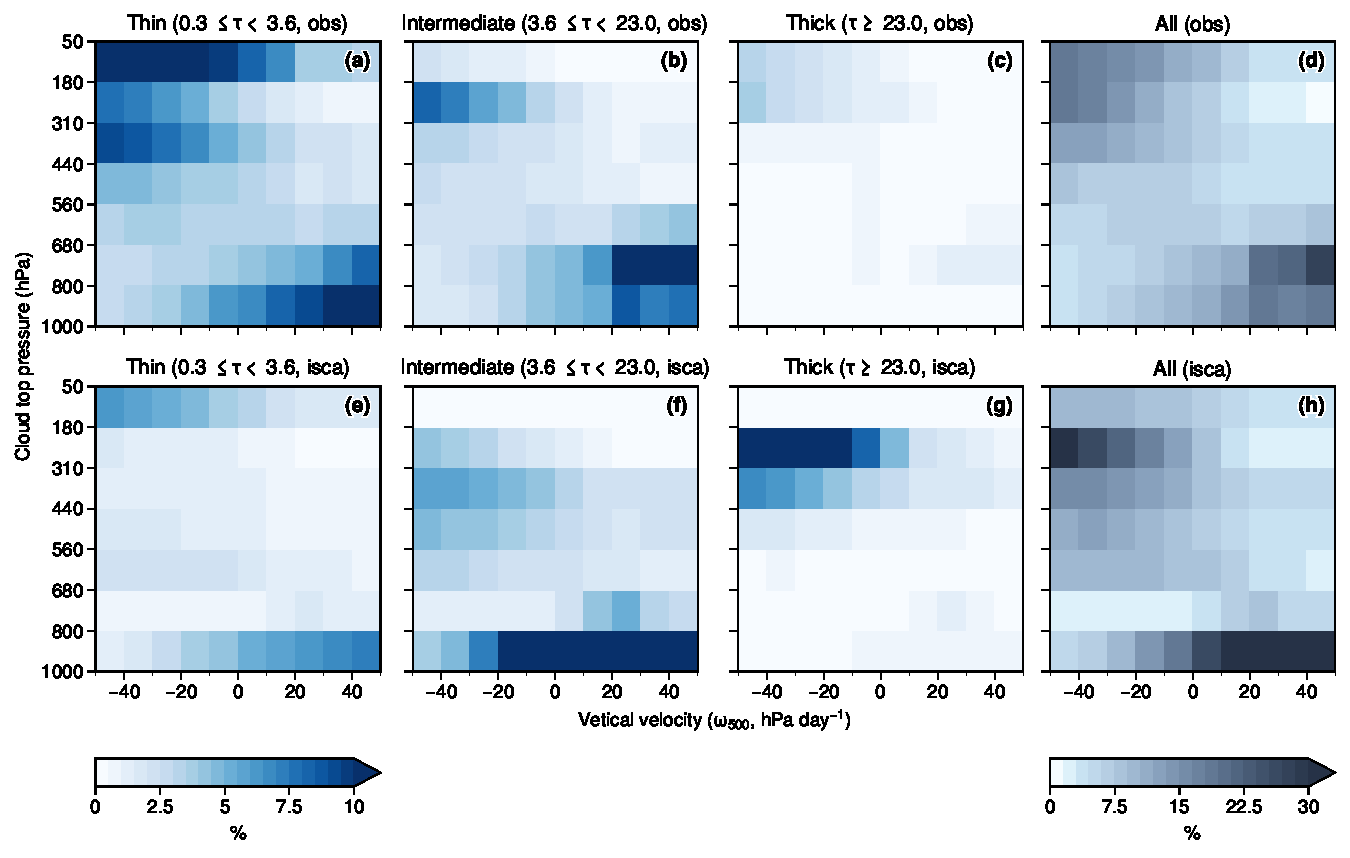
\includegraphics[width=1.0\linewidth]{{figs/change_of_CRE/clisccp_cloud_thickness_category_obs_isca_linear_sc}.pdf}
    \caption{Annual mean cloud frequency from (top row) GCM simulator-oriented ISCCP product (1998-2007) and (bottom row) one Isca simulation, sorted by vertical velocity at 500 hPa ($\omega_{500}$, units: hPa day$^{-1}$) and divided into different cloud thickness categories: (a, e) thin (0.3$\le\tau<$3.6), (b, f) intermediate (3.6$\le\tau<$23), (c, g) thick ($\tau\ge$23), and (d, h) all optical depths. For ISCCP, the $\omega_{500}$ is from ERA-Interim analysis (1998-2007). }
    \label{fig:tropical_clisccp_obs_isca}
\end{figure}

\section{Comparison of cloud feedback calculation}
\label{sec:cmp_cld_fbk_method_result}

\cite{Zelinka2013} has summarized the the diagnostic and methodology used in current studies (see their Table 1). In general, the Gregory method \citep{Gregory2004} that calculates feedback from the slope of $\Delta R$ against $\Delta T_s$ accounts for the rapid adjustments. Here $\Delta R$ is the radiative flux anomaly at the TOA and $\Delta T_s$ is the surface temperature change.  The cloud radiative effect (CRE; i.e. the all-sky minus clear-sky downward radiative flux at TOA) based method is affected by the cloud masking effect, while the cloud radiative kernel method is not affected by this masking effect.

\begin{figure}[ht]
    \centering
    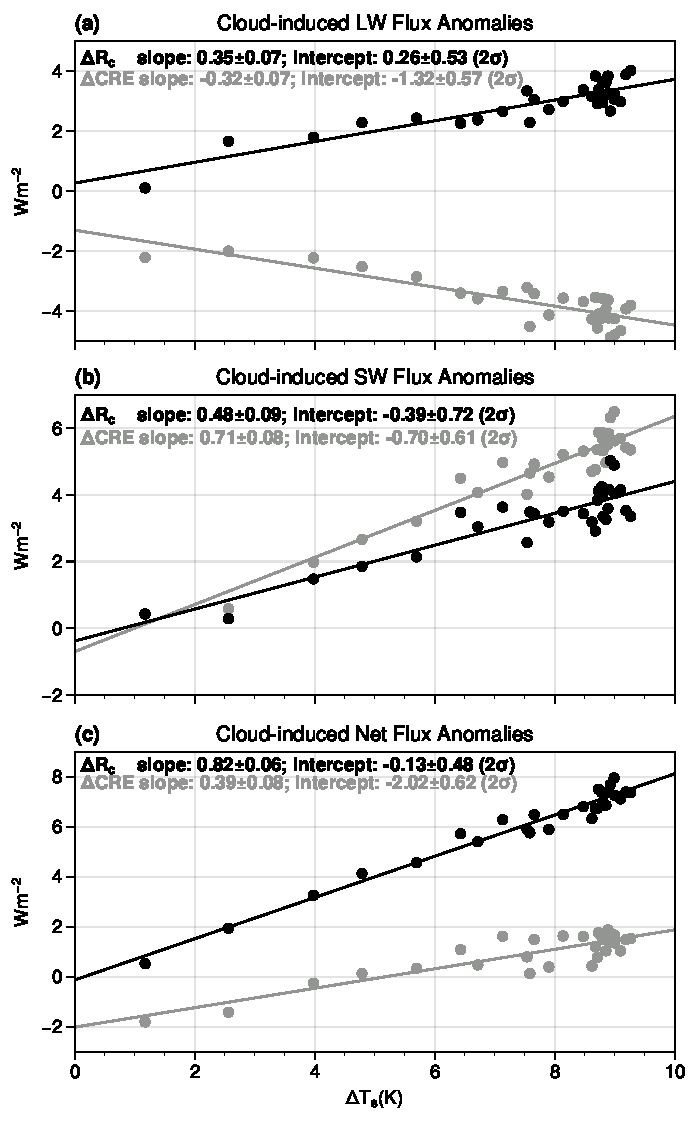
\includegraphics[width=0.6\linewidth]{{figs/change_of_CRE/gregory_plot_all_cld_fbk_v2}.pdf}
    \caption{Global and annual mean anomalies in cloud-induced TOA (a) longwave (LW), (b) shortwave (SW) and (c) net radiative flux against global mean surface temperature change ($\Delta T_s$). The black dots and lines are fluxes derived from cloud radiative kernel method \citep{Zelinka2012computing1, Zelinka2012computing2}, while the gray ones are for the cloud radiative effect (CRE).}
    \label{fig:gregory_plot_for_CRE_and_kernel_flux}
\end{figure}

Here the cloud feedback calculated from these four different methods in Isca simulations are compared and summarized as follows. \figref{fig:gregory_plot_for_CRE_and_kernel_flux} shows the Gregory plot of the global and annual mean anomalies in cloud-induced TOA radiative flux against the change in global mean surface temperature ($\Delta T_s$). These flux anomalies are estimated from CRE and cloud radiative kernel respectively, so they are corresponding to II and IV categories in Table 1 of \cite{Zelinka2013}. It is clear that there is a sign change in the slope of longwave (LW) cloud feedback (\figref{fig:gregory_plot_for_CRE_and_kernel_flux}a), where the slope changed from -0.31 Wm$^{-2}$K$^{-1}$ in category II (CRE+Gregory) to 0.35 Wm$^{-2}$K$^{-1}$ in category IV (kernel+Gregory). The LW forcing term in category II is more negative than that in category IV due to the cloud masking effect. For example, \cite{Andrews2012cloud} found that the instantaneous cloud masking effect for LW CRE is about -0.62 Wm$^{-2}$ in response to doubling CO$_2$ (see their Table 2).


The cloud feedback is also calculated according to categories I and III, and the results are in \tabref{tab:four_methods_cldfbk_results}. Focusing on the second row (the radiative kernel based diagnostic) in \tabref{tab:four_methods_cldfbk_results}, we can find that the cloud feedback parameters from two different methods (categories III and IV in Table 1 of \citealt{Zelinka2013}) are much similar, indicating that neglecting the rapid cloud adjustments has relative small impact on cloud feedback. This is also true for CRE based diagnostic (the first row in \tabref{tab:four_methods_cldfbk_results}). For example, the cloud feedback has relative small changes from category I to category II in Table 1 of \cite{Zelinka2013}. In contrast, comparing to the results from categories I and III (or categories II and IV) suggests that the cloud masking effect do have a large impact on the cloud feedback calculation. For instance, the sign of LW cloud feedback parameter changed from CRE related diagnostic to kernel-derived diagnostic.

\begin{table}[ht]
    %\begin{sidewaystable}
	\caption{Comparison of longwave (LW), shortwave (SW) and net cloud feedbacks estimated from different methods and diagnostics as summarized in Table 1 of \cite{Zelinka2013} (units: Wm$^{-2}$K$^{-1}$).}
	\vspace{0.5em}
	\centering
	\renewcommand{\arraystretch}{1.2}
	\begin{tabular}{>{\centering}m{0.4\linewidth} ccc ccc} 
	    % control width, alignment for cells
	    % https://texblog.org/2017/02/06/proper-tables-with-latex/
		\toprule
		\multirow{2}{*}{Diagnostic} & \multicolumn{3}{c}{$\Delta R/\Delta T_s$} & \multicolumn{3}{c}{\thead{Slope of $\Delta R$ against $\Delta T_s$ \\(Gregory method)}}\\
		\cline{2-4}\cline{5-7}
		 & LW & SW & Net & LW & SW & Net \\
		\midrule
		%CRE anomalies & & & & & & \\
		%Kernel-derived cloud-induced radiation anomalies & & & & & & \\
		CRE anomalies   &  -0.475 &   0.626 &    0.150 &    -0.317 &     0.706 &      0.389 \\  
        Kernel-derived cloud-induced radiation anomalies &   0.365 &   0.440 &    0.805 &     0.346 &     0.479 &      0.825 \\  
        \bottomrule
	\end{tabular}
	\label{tab:four_methods_cldfbk_results}
    %\end{sidewaystable}
\end{table}

\section{Simulated cloud feedbacks}
\label{sec:simu_cld_fbk}

\subsection{Spatial pattern}

\subsection{Zonal mean}

\begin{figure}[ht]
    \centering
    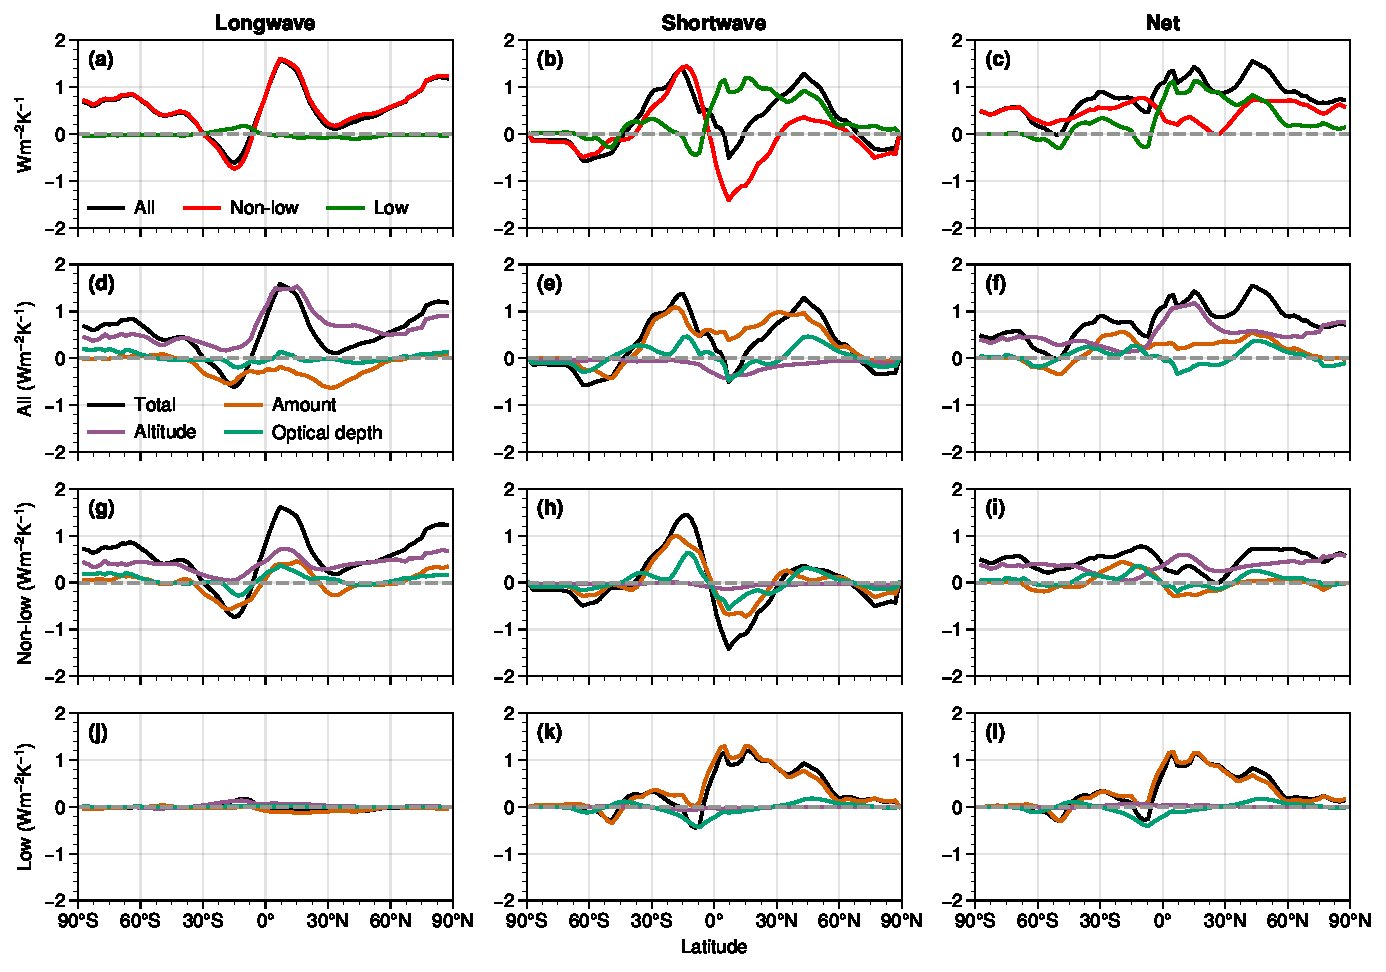
\includegraphics[width=1.0\linewidth]{{figs/change_of_CRE/annual_and_zonal_mean_cld_fbk}.pdf}
    \caption{Zonal and ensemble mean (left column) longwave, (middle column) shortwave, and (right column) net cloud feedbacks from Isca perturbed parameter ensemble. (a-c) Total cloud feedbacks and their separate contributions from non-low (red) and low (green) clouds. Total cloud feedbacks (black) and their amount (orange), altitude (purple), and optical depth (green) components for (d-f) all clouds, (g-i) non-low clouds only, and (j-l) low clouds only.}
    \label{fig:zonal_mean_cld_fbk_ensemble}
\end{figure}


\section{Spread of cloud feedback}
\label{sec:spread_of_cld_fbk_in_PPE}

\subsection{Spread of global mean cloud feedbacks}
\label{sec:spread_of_gm_cld_fbks_PPE}

\begin{figure}[ht]
    \centering
    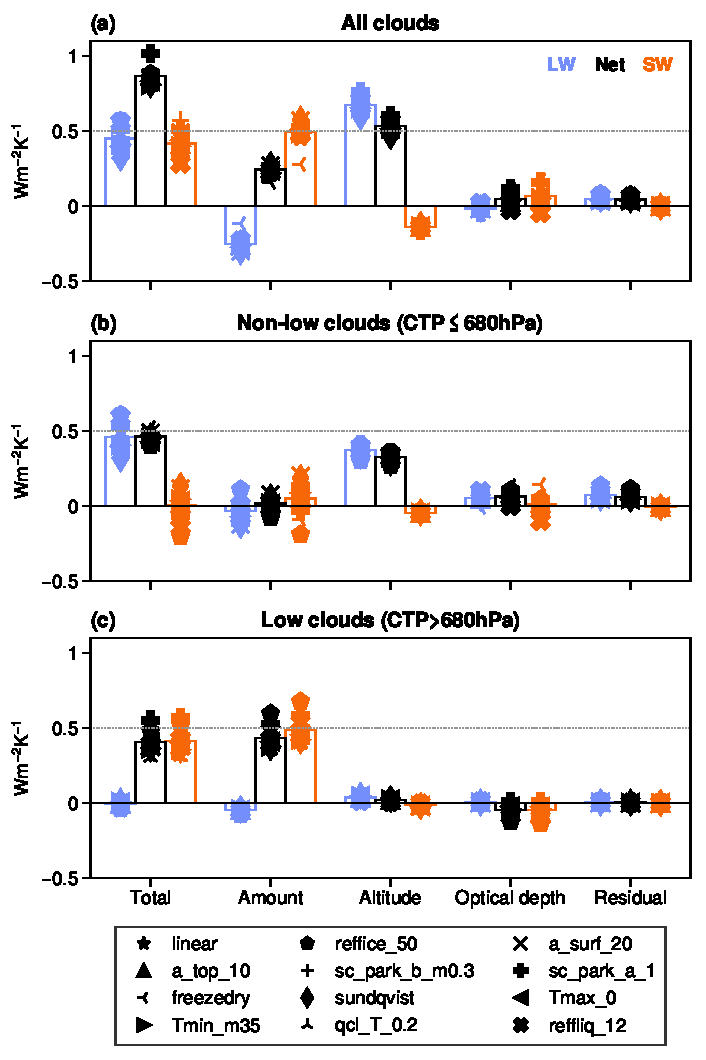
\includegraphics[width=0.8\linewidth]{{figs/change_of_CRE/global_mean_cld_fbk_decomp_scatter}.pdf}
    \caption{Global mean (orange) shortwave (SW), (blue) longwave (LW), and (black) net cloud feedbacks decomposed into amount, altitude, optical depth, and residual components for (a) all clouds, (b) non-low clouds (cloud top pressure, CTP$\le$680 hPa ), and (c) low clouds (CTP > 680hPa). The mean feedbacks of perturbed parameter ensemble are shown as empty bars.}
    \label{fig:global_mean_cld_fbk_scatter}
\end{figure}


\subsection{Comparison with WCRP assessment}
\label{sec:cmp_with_Sherwood_assessment}

\begin{figure}[ht]
    \centering
    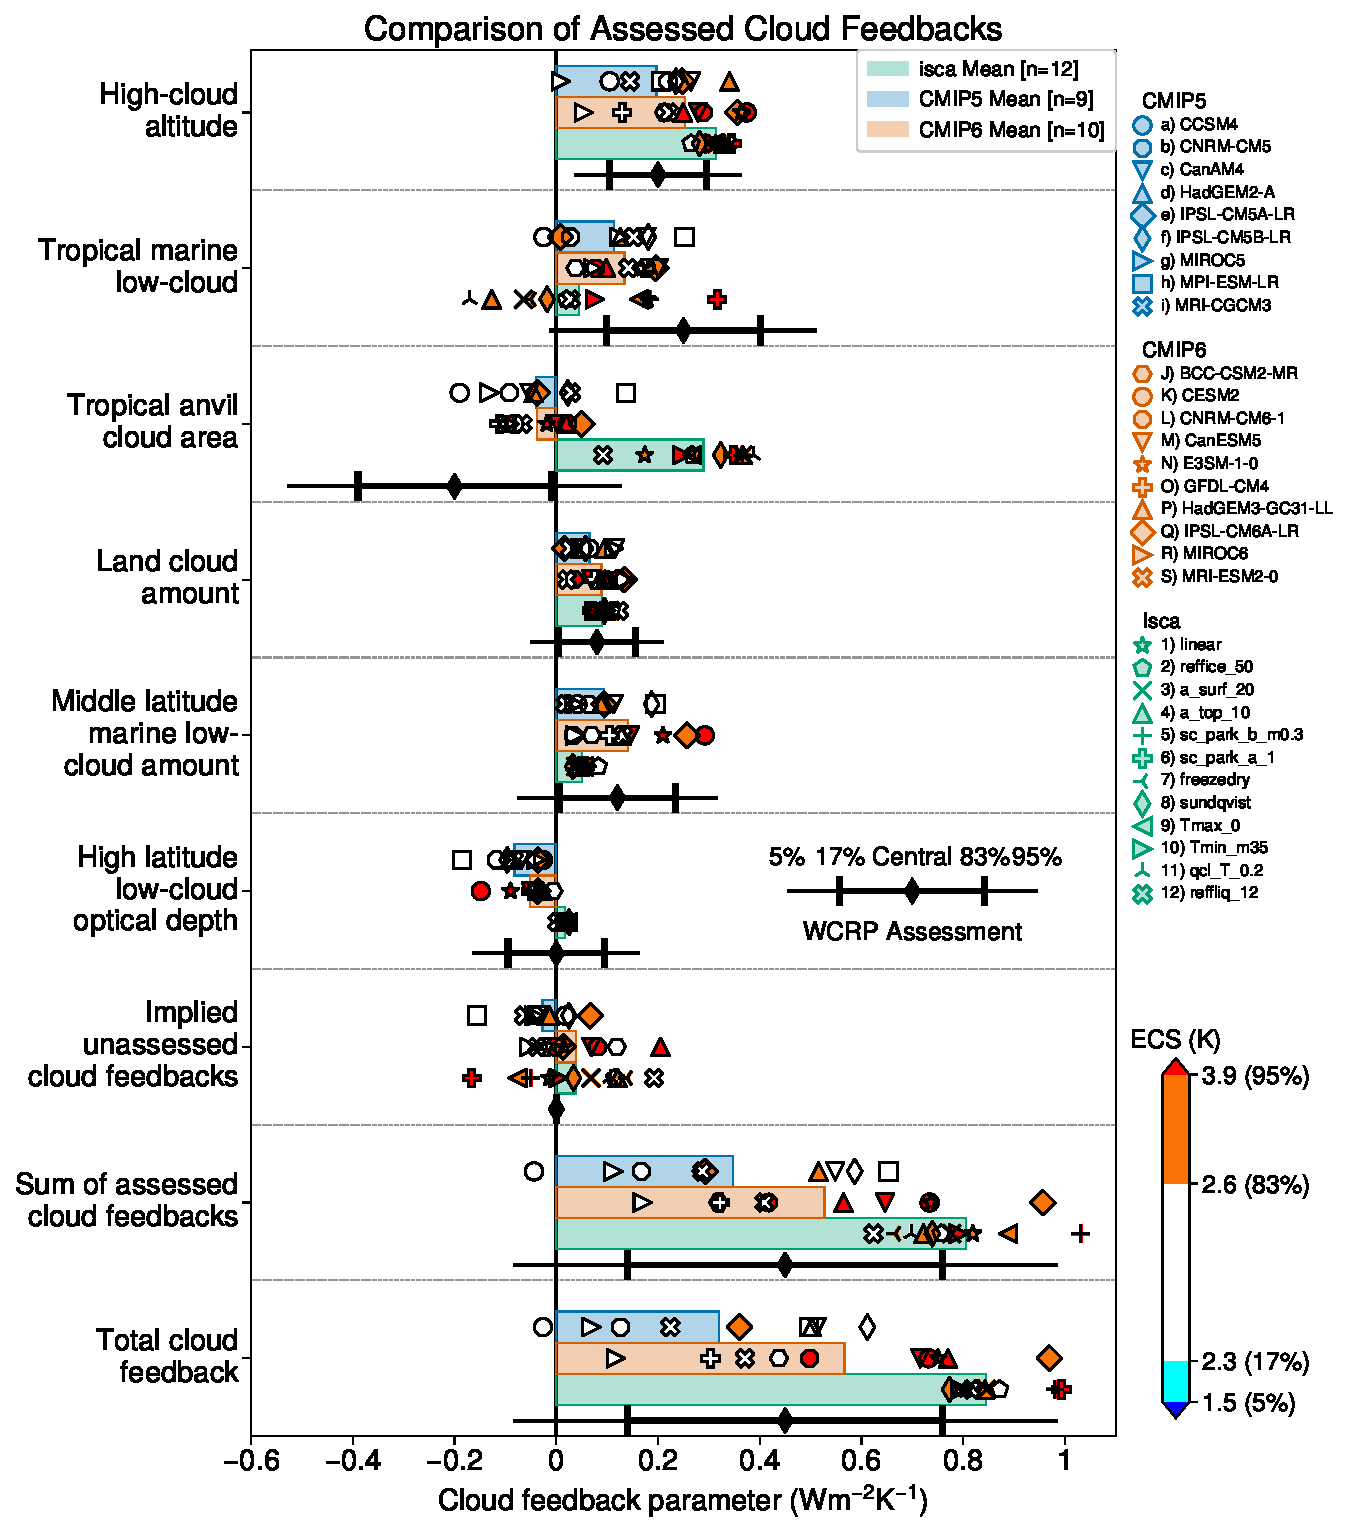
\includegraphics[width=1\linewidth]{{figs/change_of_CRE/WCRP_assessed_cld_fbks_amip-p4K}.pdf}
    \caption{Cloud feedback components estimated from climate model simulations and as assessed in \cite{Sherwood2020}. For each component, the individual model values are indicated with symbols, the multi-model means are indicated with blue (CMIP5), orange (CMIP6) and green (Isca) bars, and the expert assessed \textit{likely} (66\%, or 17\%--83\%) and \textit{very likely} (90\%, or 5\%--95\%) confidence intervals are indicated with thick and thin black errorbars, respectively. Model symbols (only for CMIP5/6) are color-coded by equilibrium climate sensivity (ECS) with color boundaries corresponding to the edges of the \textit{likely} (17\%--83\%) and \textit{very likely} (5\%--95\%) ranges of the Baseline posterior probability density function (PDF) of  ECS from \cite{Sherwood2020}. The results from Isca simulation are added to original Fig. 1 of \cite{Zelinka2021evaluating}.}
    \label{fig:WCRP_assessment}
\end{figure}

\cite{Zelinka2021evaluating} evaluated the cloud feedbacks from CMIP5 and CMIP6 models and compared them to the latest World Climate Research Programme (WCRP) assessment of cloud feedbacks reported in \cite{Sherwood2020}. Note that only 9 CMIP5 and 10 CMIP6 models are used, as only those that have successfully implemented the COSP \citep{BodasSalcedo2011} are adopted. Based on the analysis from \cite{Zelinka2021evaluating}, here the perturbed parameter ensemble simulations from Isca simulations are also added to this comparison, as shown in \figref{fig:WCRP_assessment}. In this figure, the feedback values from each category are weighted averaged according to their area fractions, so that the values shown in the last row of the figure are the direct sum of these categories. 

All the simulated cloud feedbacks from Isca are with the \textit{very likely} (90\%, or 5\%--95\%; thin black line of WCRP assessment) confidence intervals of expert assessment, except the ones related to tropical anvil cloud area and tropical marine low cloud. In Isca simulations, the tropical anvil cloud area feedback (third row) is computed as the sum of non-altitude related feedbacks from both low and high clouds in tropical deep convection region. Specifically, the sum includes low and high cloud mount and optical depth feedbacks. This feedback is strongly positive with the mean value larger than 0.3 Wm$^{-2}$K$^{-1}$, while the mean value of expert assessment is -0.2 Wm$^{-2}$K$^{-1}$ (1-$\sigma$ uncertainty is 0.2 Wm$^{-2}$K$^{-1}$). This feature makes the total cloud feedback from Isca simulations much positive, and are located at the right end of expert assessment (last row). Note that the CMIP5 and CMIP6 models also underestimate the magnitude of tropical anvil cloud area feedback, and some also produce the positive feedback parameters for this category. Nevertheless, their ensemble mean has the same negative sign as the expert assessment, although we notice it is very weak and close to zero. 

Regarding to the tropical marine low cloud feedback, the ensemble mean feedback from Isca simulation is much weaker than the expert assessed, and also weaker than the ensemble mean of CMIP5/6 models. Another feature of Isca simulation for this category is that the spread is quite large, and some member even produce the negative marine low cloud feedback. This is possibly due to...

%In addition, the \textit{likely} (66\%, or 17\%--83\%) and \textit{very likely} (90\%, or 5\%--95\%) confidence intervals from expert assessments of cloud feedbacks \citep[see Table 1 of][]{Sherwood2020} are indicated by the 

\figref{fig:WCRP_assessment} is produced using the software package developed by \cite{Zelinka2021evaluating}, available at \url{https://github.com/mzelinka/assessed-cloud-fbks}.

\subsection{Regional contributions}
\label{sec:reg_contri_to_spread_of_cldfbk}

\subsection{Cloud controlling factor analysis}
\label{sec:cld_control_factor}


\section{Implications for equilibrium climate sensitivity}
\label{sec:implification_for_ECS}


\section{Summary and discussion}